\documentclass[a4paper, 12pt]{article}%тип документа

%отступы
\usepackage[left=2cm,right=2cm,top=2cm,bottom=3cm,bindingoffset=0cm]{geometry}

%Русский язык
\usepackage[T2A]{fontenc} %кодировка
\usepackage[utf8]{inputenc} %кодировка исходного кода
\usepackage[english,russian]{babel} %локализация и переносы

%Вставка картинок
\usepackage{wrapfig}
\usepackage{graphicx}
\graphicspath{{images/}}
\DeclareGraphicsExtensions{.pdf,.png,.jpg}

%оглавление
\usepackage{titlesec}
\titlespacing{\chapter}{0pt}{-30pt}{12pt}
\titlespacing{\section}{\parindent}{5mm}{5mm}
\titlespacing{\subsection}{\parindent}{5mm}{5mm}
\usepackage{setspace}

\newcommand{\eds}{\ensuremath{ \mathscr{E}}}
\newcommand{\be}{\ensuremath{\beta}}

%Графики
\usepackage{multirow}
\usepackage{pgfplots}
\pgfplotsset{compat=1.9}

%Математика
\usepackage{amsmath, amsfonts, amssymb, amsthm, mathtools}

%Стиль страницы
\usepackage{fancyhdr}
\pagestyle{fancy}

\begin{document}

\begin{titlepage}

\begin{center}
%\vspace*{1cm}
\large\textbf{Московский Физико-Технический Институт}\\
\large\textbf{(государственный университет)}
\vfill
\line(1,0){430}\\[1mm]
\huge\textbf{Работа 5.4.2}\\
\line(1,0){430}\\[1mm]
\vfill
\large Сибгатуллин Булат, ФРКТ\\
\end{center}

\end{titlepage}
\fancyhead[L] {Работа 5.4.2}
\noindent \textbf{Цель работы:} \\
\indent С помощью магнитного спектрометра исследовать энергетический спектр $\beta$ - частиц при распаде ядер $^{137}$Cs  и определить их максимальную энергию.

\section{Описание работы} 

Бета-распадом называется самопроизвольное превращение ядер, при котором их массовое число не изменяется, а заряд увеличивается или уменьшается на единицу. Бета-активные ядра встречаются во всей области значений массового числа A, начиная от единицы (свободный нейтрон) и кончая самыми тяжелыми ядрами. Период полураспада $\beta$ - активных ядер изменяется от ничтожных долей секунды до $10^{18}$ лет. Выделяющаяся при единичном акте $\beta$ - распада энергия варьируется от 18 кэВ до 13,4 МэВ.

В данной работе мы будем иметь дело с электронным распадом

\begin{equation}\label{}
^A_ZX \rightarrow ^{\; \; \; \; \: A}_{Z+1}X + e^- + \widetilde{\nu}
\end{equation}

при котором кроме электрона испускается антинейтрино. Освобождающаяся при $\beta$-распаде энергия делится между электроном, антинейтрино и дочерним ядром, однако доля энергии, передаваемой ядру, исчезающе мала по сравнению с энергией, уносимой электроном и антинейтрино. Практически можно считать, что эти две частицы делят между собой всю освобождающуюся энергию. Поэтому электроны могут иметь любое значение энергии  от нулевой до некоторой максимальной, которая равна энергии, освобождающейся при $\beta$-распаде, являющейся важной физической величиной.

Вероятность $ dw $ того, что при распаде электрон вылетит с импульсом в интервале $d^3p$, а антинейтрино с импульсом в интервале $d^3k$, пропорциональна произведению этих дифференциалов. Но мы должны еще учесть закон сохранения энергии, согласно которому импульсы $ p $ и $ k $ электрона и антинейтрино связаны соотношением

\begin{equation}
E_e - E - ck = 0,
\end{equation}

где $E_e$ - максимальная энергия электрона, кинетическая энергия электрона $ E $ связана с его импульсом обычным релятивистским соотношением

\begin{equation}
E = c\sqrt{p^2 + m^2c^2} - mc^2,
\end{equation}

а через $ ck $ обозначена энергия антинейтрино с импульсом $ k $. Условие можно учесть введением в выражение для $ dw $ $\delta$ - функции
\begin{equation}
\delta (E_e - E - ck).
\end{equation}

Таким образом, вероятность $ dw $ может быть записана в виде

\begin{equation}\label{dw}
dw = D \delta (E_e - E - ck)d^3 p d^3 k = D \delta (E_e - E - ck)p^2dpk^2dkd{\Omega}_ed{\Omega}_{\widetilde{\nu}},
\end{equation}

где $ D $ --- некоторый коэффициент пропорциональности, $d\Omega_e$ , $d\Omega_{\widetilde{\nu}}$ --- элементы телесных углов направлений вылета электрона и нейтрино. Вероятность $ dw $ непосредственно связана с $\beta$-спектром, поскольку для большого числа $N_0$ распадов число $dN$ распадов с вылетом электрона и антинейтрино с импульсом соответственно от $ p $ до $ p + dp $ и от
$ k $ до $ k + d $k определяется соотношением

\begin{equation}\label{dn = n_0 dw}
dN = N_0 dw  
\end{equation}

Коэффициент $ D $ в формуле \eqref{dw} можно считать для рассматриваемых нами так называемых разрешенных фермиевских типов распадов с хорошей точностью константой (разрешенными называются такие переходы, при которых не изменяются ни момент, ни четность состояния ядра). В этом случае величину $ dw $ из \eqref{dn = n_0 dw} можно проинтегрировать по всем углам и по абсолютному значению импульса нейтрино.

После умножения на полное число распадов $ N $ проинтегрированное выражение приобретает смысл числа электронов $ dN $, вылетающих из ядра с импульсом, абсолютная величина которого лежит между $ p $ и$  p + dp $:

\begin{equation}\label{dN}
dN = \dfrac{16\pi^2 N_0}{c^2}Dp^2(E_e - E)^2dp.
\end{equation}

Чтобы получить распределение электронов по энергиям, надо в \eqref{dN} перейти от $ dp $ к $ dE $:

\begin{equation}
dE = \dfrac{c^2p}{E + mc^2}dp,
\end{equation}

после чего выражающая форму $\beta$ --- спектра величина $ N(E) = dN/dE $
приобретает вид

\begin{equation}\label{dN/dE big}
\dfrac{dN}{dE} = N_0Bcp(E + mc^2)(E_e - E)^2 = N_0B\sqrt{E(E + 2mc^2)}(E_e - E)^2(E + mc^2)
\end{equation}

где $B = (16\pi^2/c^4)D$. В нерелятивистском приближении, которое и имеет место с нашем случае, выражение \eqref{dN/dE big} упрощается, и мы имеем

\begin{equation}\label{dN/dE}
\dfrac{dN}{dE} \approx \sqrt{E}(E_e - E)^2.
\end{equation}

\begin{wrapfigure}[12]{l}{0.35\linewidth}
	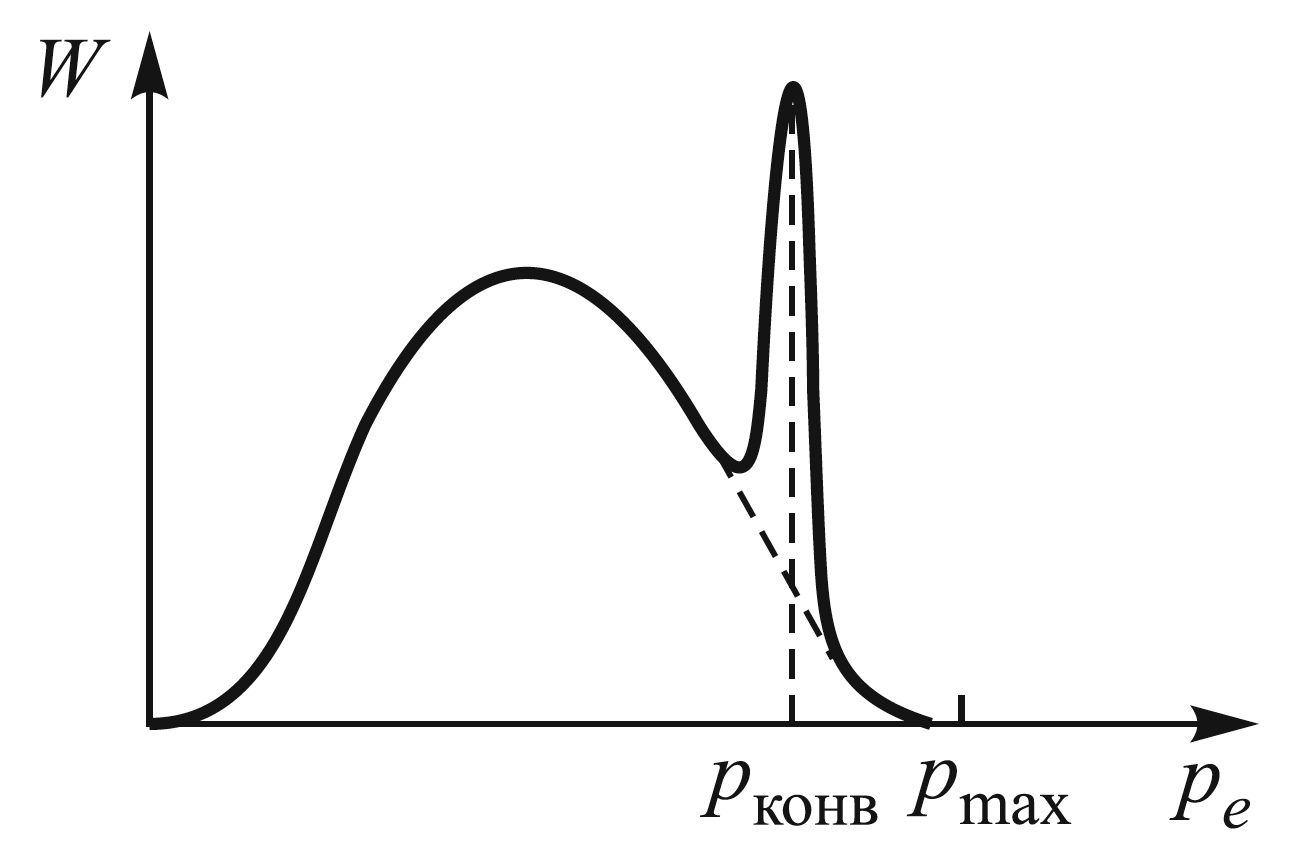
\includegraphics[width=\linewidth]{spektr}
	\caption{Форма спектра \be-частиц при разрешенных переходах}
	\label{ris spetr}
\end{wrapfigure}


Выражение \eqref{dN/dE} приводит к спектру, имеющему вид широкого колокола (рис \ref{ris spetr}). Кривая плавно отходит от нуля и столь же плавно, по параболе, касается оси абсцисс в области максимальной энергии электронов $E_e$. 

Дочерние ядра, возникающие в результате $\beta$-распада, нередко оказываются возбужденными. Возбужденные ядра отдают свою энергию либо излучая $\gamma$-квант (энергия которого равна разности энергий начального и конечного уровней), либо передавая избыток энергии одному из электронов с внутренних оболочек атома. Излучаемые в таком процессе электроны имеют строго определенную энергию и называются конверсионными.

Конверсия чаще всего происходит на оболочках $ K $ или $ L $. На спектре, представленном на рис. \ref{ris spetr}, видна монохроматическая линия, вызванная электронами конверсии. Ширина этой линии в нашем случае является чисто аппаратурной, по ней можно оценить разрешающую силу спектрометра.


\section{Экспериментальная установка}
	
	Для определения энергии $\beta$-частиц в работе используется магнитный спектрометр, схема которого показана на рисунке \ref{pic:scheme} слева. Электроны испускаются радиоактивным источником и попадают в магнитное поле катушки, ось которой параллельна $OZ$. Траектории электронов сходятся в одной точке --- фокусе, где и установлен сцинтилляционный счетчик, сигналы которого усиливаются фотоумножителем и регистрируются пересчетным прибором. Фокусное расстояние $f$ магнитной линзы связано с током в катушке $I$ и импульсом $p_e$ регистрируемых частиц следующим образом:
	
	\[ \frac{1}{f} \propto \frac{I^2}{p_e^2} \]  
	
	При неизменной геометрии установки, увеличивая и уменьшая силу тока, можно фокусировать электроны разных импульсов, причем 
	
	\begin{equation}\label{k}
	p_e = kI,
	\end{equation}
	
	 где $k$ --- коэффициент пропорциональности, являющийся параметром установки.

	\begin{figure}[h]
	\centering
	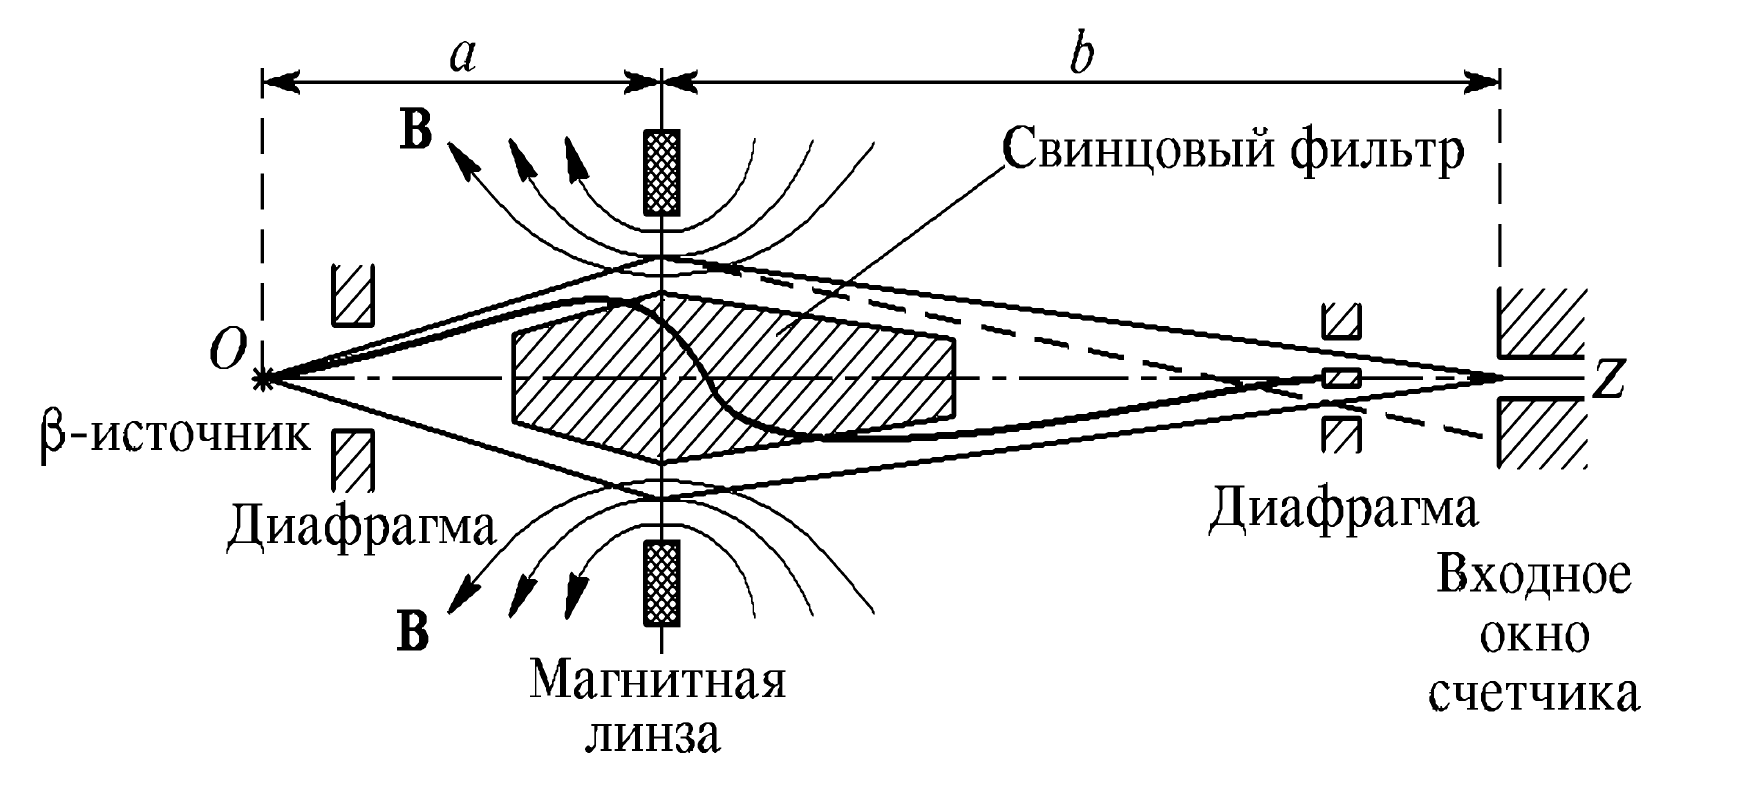
\includegraphics[width=0.48\textwidth]{lab}
	\hfill
	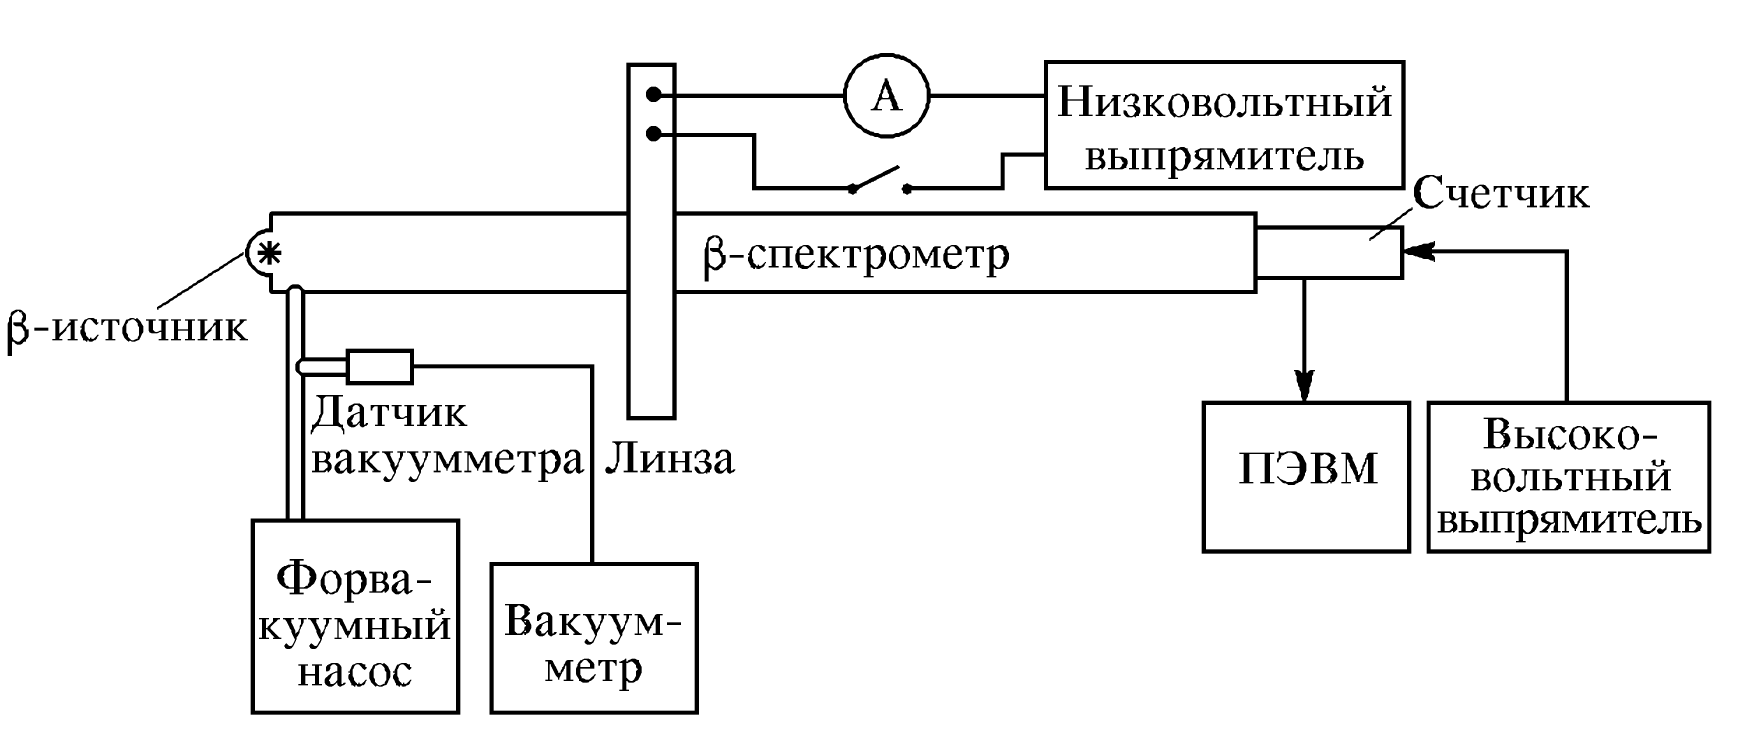
\includegraphics[width=0.48\textwidth]{lab2}
	\caption{слева --- схема $\beta$-спектрометра; справа --- блок-схема установки для изучения спектра}
	\label{pic:scheme}
\end{figure}

В $\beta$-спектрометре установлены диафрагмы для ограничения углов вылета частиц из источника и свинцовый фильтр для защиты от прямого попадания $\gamma$-лучей. 

Число частиц $N$, регистрируемых на установке, равно: $N \approx W \cdot \Delta p_e$, где $\Delta p_e$ - разрешающая способность спектрометра. Дифференцируя выражение для форуса магнитной линзы, получим: $\Delta p_e = \frac{1}{2}\frac{\Delta f}{f}p_e$, то есть $\Delta p_e \propto p_e$. Таким образом, для количества частиц справедлива формула: 

\begin{equation}\label{N}
 N = CW(p_e)p_e 
\end{equation}

Здесь $C$ - некоторая константа.

\section{Выполнение работы}

\begin{enumerate}
\item Включим пересчетный прибор, высоковольтный выпрямитель и вакуумметр. Если показания вакуумметра заметно превышают 0,1 Тор, включим форвакуумный насос и откачаем спектрометр. Затем отключим насос, не забыв соединить его с атмосферой.

\item Установим рабочее напряжение на ФЭУ.

\item Для того, чтобы убедиться, что \be-спектрометр действительно работает убедимся, что скорость счета зависит от величины тока в катушке.

\item Выключим ток в линзе и с точностью 2-3$\%$ измерим фоновый счет спектрометра. Измерения фона повторим в середине и в конце опыта.

\item Проведем предварительные измерения, изменяя силу тока в фокусирующей катушке каждый раз на 0,2 А и записывая число счетов за 100 с. Затем уточним измерения в области спада спектральной кривой и в районе конверсионного пика, изменяя ток с шагом в 0,1 А.

\item Занесем получившиеся данные в таблицу и также добавим в таблицу откалиброванные значения с учетом того, что $p_{conv}\cdot c = 1013,5$ кэВ, а энергия электроново внутренней конверсии $^{137}Cs$ равна $E_{conv} = 624$ кэВ. Сила тока, при которой наблюдается конверсионный пик равна 4,25 А. Зная это запишем данные в таблицу:

\begin{figure}[h]
    \centering
    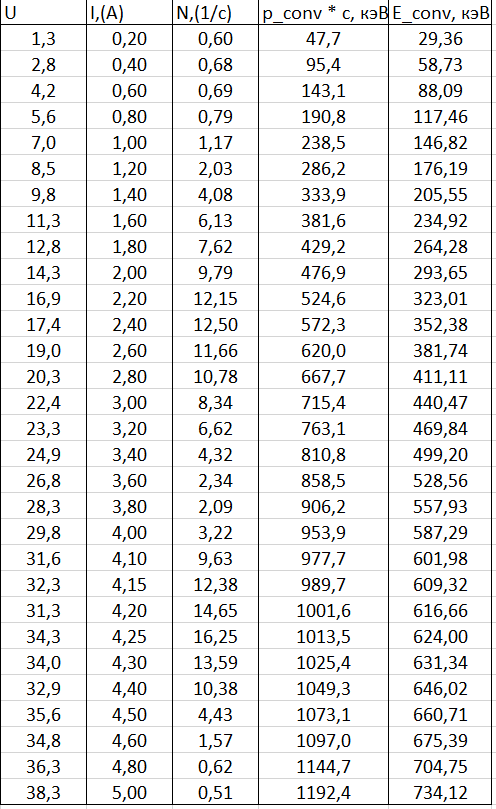
\includegraphics[width=0.8\linewidth]{table_1.PNG}
    \caption{Измеренные данные}
    \label{fig:table_1}
\end{figure}

По полученным данным построим спектр $\beta$-распада атома $^{137}Cs$:

\begin{figure}[h]
    \centering
    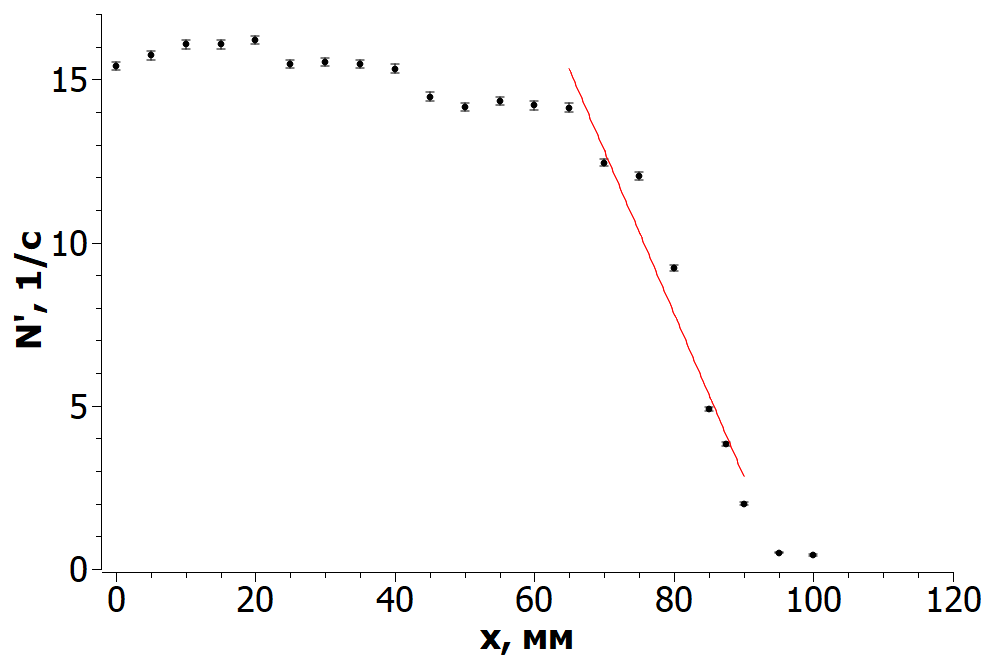
\includegraphics[width=0.8\linewidth]{graph_1.PNG}
    \caption{Спектр $\beta$-распада атома $^{137}Cs$}
    \label{fig:graph_1}
\end{figure}

\item Сдвиг графика по оси ординат сделаем на величину радиационного фона при $I = 5$ А. По этим данным построим откалиброванный график $N(p)$:

\begin{figure}[h]
    \centering
    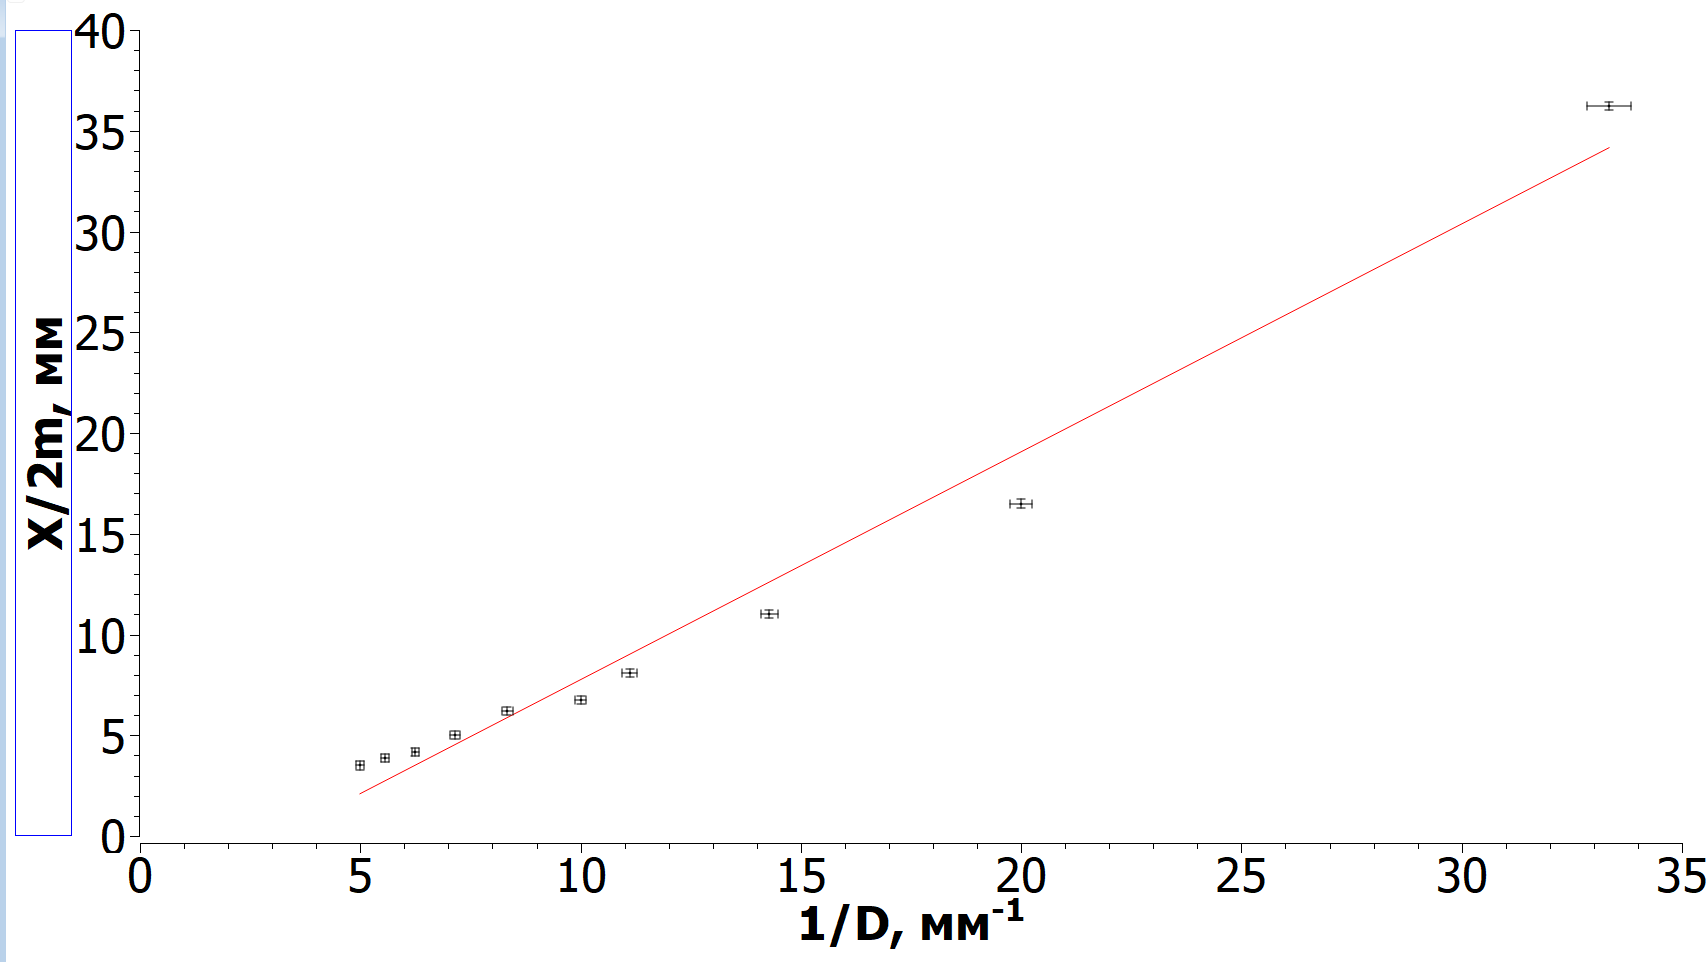
\includegraphics[width=0.8\linewidth]{graph_2.PNG}
    \caption{Спектр $\beta$-распада атома $^{137}Cs$}
    \label{fig:graph_2}
\end{figure}

\item Определим максимальную энергию $\beta$-спектра. Для этого мы отложим по оси ординат величину $\sqrt{N}/p^{3/2}$, а по оси абсцисс энергию $\beta$-частиц (с учётом того, что энергия электронов внутренней конверсии $^{137}$Cs равна 634, кэВ). В таком случае мы задействуем большинство экспериментальных точек, и прежде всего точки середины $\beta$-спектра, которые измерены с наилучшей точностью.

\begin{figure}[h]
    \centering
    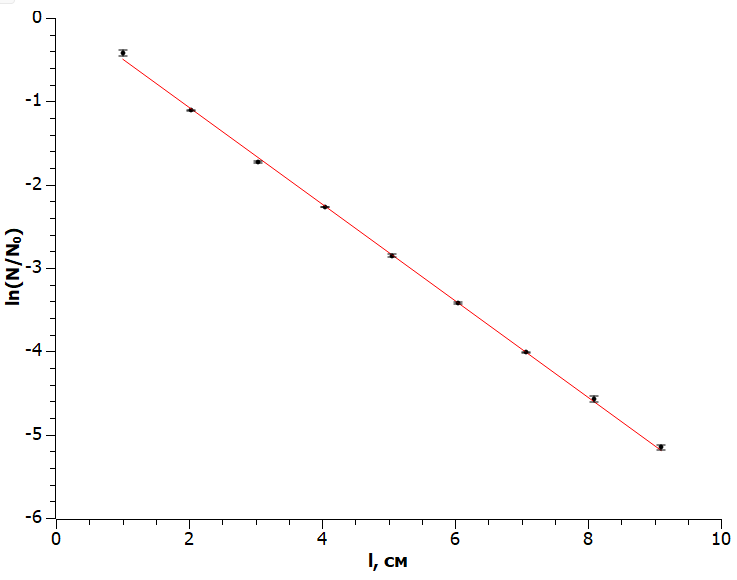
\includegraphics[width=0.8\linewidth]{graph_3.PNG}
    \caption{График Ферми-Кюри.}
    \label{fig:graph_2}
\end{figure}

\begin{center}
		\begin{table}
			\caption{Результаты линейной аппроксимации.}
			\label{table:Emax}
			\begin{tabular}{|c|c|c|}
				\hline
				& $a$, $10^5 * \text{с}^{1/2} \cdot {c^{3/2}} \cdot\text{кэВ}^{-5/2}$ & $b$, $10^5 * \text{с}^{1/2} \cdot {c^{3/2}} \cdot\text{кэВ}^{-3/2}$ \\ \hline
							Величина    & -0,0966                                                        & 58,0                                                                     \\ \hline
							Погрешность & 0,0046                                                         & 1,8                                                                     \\ \hline
						\end{tabular}
		\end{table}
\end{center}

Ясно, что $E_m = - \frac{b}{a}$ и $\sigma_{E_m} = E_m \sqrt{\left(\frac{\sigma_a}{a}\right)^2 + \left(\frac{\sigma_b}{b}\right)}$, откуда $E_m =(600 \pm 34) \ \text{кэВ}.$

\end{enumerate}

\section{Вывод}
	В ходе лабораторной работы с помощью магнитного спектрометра мы исследовали энергетический спектр $\beta$-частиц при распаде ядер $^{137}$Cs. Калибровку спектрометра осуществили по энергии электронов внутренней конверсии.
	
	Также мы определили максимальную энергию $E_m = 600$ кэВ вылетающих электронов при $\beta$-распаде ядря $^{137}$Cs методом Ферми-Кюри  с ошибкой в 5,6\%.

\end{document}